
% Masters/Doctoral Thesis 
% LaTeX Template
% Version 2.5 (27/8/17)
%
% This template was downloaded from:
% http://www.LaTeXTemplates.com
%
% Version 2.x major modifications by:
% Vel (vel@latextemplates.com)
%
% This template is based on a template by:
% Steve Gunn (http://users.ecs.soton.ac.uk/srg/softwaretools/document/templates/)
% Sunil Patel (http://www.sunilpatel.co.uk/thesis-template/)
%
% Template license:
% CC BY-NC-SA 3.0 (http://creativecommons.org/licenses/by-nc-sa/3.0/)
%
%%%%%%%%%%%%%%%%%%%%%%%%%%%%%%%%%%%%%%%%%

%----------------------------------------------------------------------------------------
%	PACKAGES AND OTHER DOCUMENT CONFIGURATIONS
%----------------------------------------------------------------------------------------

%Notes

% Related work - tabelen übersicht über frntend etc. , "das hab ich bentutz" in implementation reinballern  X
%bei POC und MVP itemize statt überschrift, ab halbe seite pro thema überschrift ok X
%summary am ende von related work - immer individuelle lösungen, viel open source, gibt standart
% am ende sagen gibt keine standarts, wär nice.
%POC fehleranfälligkeit, effizienz, zeitaufwand X
%Gateway funktionalität in UML reinpacken, Rätsel als eigenständige pakete klarer hervoherben
%Neue Bereiche farbig markieren


% bei den overviews How/ restrictions aufteilen statt why/not
%Change gui statt node editor bei challenges, future developments (ideas) x
%kosten nutzen rechnung theoretisch überlegeung, messen
%Vorher nachher tabelle workload vergleich pfeile die verbesserung darstellen x
%Für unteraspekte
%Weniger absätze, absätze zusammenfassen

%Limitations projekt selber vs Ich und die arbeit

%Conclusion beantwortet was in der einleitung gestellt wurde,
%Einleitung mehr motivation herausforerung 
%Allgemeine Ebene conclusion forschungsbereich iot kein standart 
%da iot große rolle spielen wird standartisierung von iot wichitg in jedem iot kontext prozesse verieinfacht werden können 
% indem projekt wär cooler gewesen wenns standataisiert worden wäre, in dem porjekt haben 
%ey ich mach meine abgabe späte rwiel time knapp, kollqoum anfang januar lets do it
%chance geben feedback zu geben
%

\documentclass[
11pt, % The default document font size, options: 10pt, 11pt, 12pt
oneside, % Two side (alternating margins) for binding by default, uncomment to switch to one side
english, % ngerman for German
onehalfspacing, % Single line spacing, alternatives: onehalfspacing or doublespacing
%draft, % Uncomment to enable draft mode (no pictures, no links, overfull hboxes indicated)
%nolistspacing, % If the document is onehalfspacing or doublespacing, uncomment this to set spacing in lists to single
%liststotoc, % Uncomment to add the list of figures/tables/etc to the table of contents
%toctotoc, % Uncomment to add the main table of contents to the table of contents
parskip, % Uncomment to add space between paragraphs
%nohyperref, % Uncomment to not load the hyperref package
headsepline, % Uncomment to get a line under the header
%chapterinoneline, % Uncomment to place the chapter title next to the number on one line
%consistentlayout, % Uncomment to change the layout of the declaration, abstract and acknowledgements pages to match the default layout
]{MastersDoctoralThesis} % The class file specifying the document structure

\usepackage[utf8]{inputenc} % Required for inputting international characters
\usepackage[T1]{fontenc} % Output font encoding for international characters
%\usepackage{enumitem}
\usepackage{mathpazo} % Use the Palatino font by default
\usepackage{url}
\usepackage[nobottomtitles*]{titlesec}
\usepackage{rotating}
\usepackage{caption, copyrightbox}
\usepackage{float}
\usepackage{hyperref}
\usepackage{amsmath}


\usepackage[
    backend=biber,
    style=numeric,
	natbib=true,
	sorting= none,
	url=true, 
	urldate=long,
    doi=true,
	eprint=true,
]{biblatex}


\addbibresource{example.bib} % The filename of the bibliography

\usepackage[autostyle=true]{csquotes} % Required to generate language-dependent quotes in the bibliography

\DeclareSourcemap{
    \maps{
        \map[overwrite]{
            \step[fieldsource=urldate,
            match=\regexp{([0-9]{2})\.([0-9]{2})\.([0-9]{4})},
            replace={$3-$2-$1},
            final]
        }
    }
}


%----------------------------------------------------------------------------------------
%	MARGIN SETTINGS
%----------------------------------------------------------------------------------------
\geometry{
	paper=a4paper, % Change to letterpaper for US letter
	inner=2.5cm, % Inner margin
	outer=3.8cm, % Outer margin
	bindingoffset=.5cm, % Binding offset
	top=1.5cm, % Top margin
	bottom=1.5cm, % Bottom margin
	%showframe, % Uncomment to show how the type block is set on the page
}


%Depth of Table of contents 
\setcounter{tocdepth}{1}


%----------------------------------------------------------------------------------------
%	THESIS INFORMATION
%----------------------------------------------------------------------------------------

\thesistitle{Development of an Integration Platform for IoT Devices} % Your thesis title, this is used in the title and abstract, print it elsewhere with \ttitle
\supervisor{Dr. Christian  \textsc{Geiger}} % Your supervisor's name, this is used in the title page, print it elsewhere with \supname
\examiner{Dr. Manfred Wojciechowski} % Your examiner's name, this is not currently used anywhere in the template, print it elsewhere with \examname
\degree{Bachelor of Engineering} % Your degree name, this is used in the title page and abstract, print it elsewhere with \degreename
\author{Cara \textsc{Watermann}} % Your name, this is used in the title page and abstract, print it elsewhere with \authorname
\addresses{} % Your address, this is not currently used anywhere in the template, print it elsewhere with \addressname

\subject{Medientechnik} % Your subject area, this is not currently used anywhere in the template, print it elsewhere with \subjectname
\keywords{} % Keywords for your thesis, this is not currently used anywhere in the template, print it elsewhere with \keywordnames
\university{\href{http://www.university.com}{Hochschule Düsseldorf}} % Your university's name and URL, this is used in the title page and abstract, print it elsewhere with \univname
\department{\href{http://department.university.com}{Media Technology}} % Your department's name and URL, this is used in the title page and abstract, print it elsewhere with \deptname
\group{\href{http://researchgroup.university.com}{Research Group Name}} % Your research group's name and URL, this is used in the title page, print it elsewhere with \groupname
\faculty{\href{http://faculty.university.com}{Media}} % Your faculty's name and URL, this is used in the title page and abstract, print it elsewhere with \facname

\AtBeginDocument{
\hypersetup{pdftitle=\ttitle} % Set the PDF's title to your title
\hypersetup{pdfauthor=\authorname} % Set the PDF's author to your name
\hypersetup{pdfkeywords=\keywordnames} % Set the PDF's keywords to your keywords
\hypersetup{linkcolor=black}% make the links black

}

\begin{document}

\frontmatter % Use roman page numbering style (i, ii, iii, iv...) for the pre-content pages

\pagestyle{plain} % Default to the plain heading style until the thesis style is called for the body content

%----------------------------------------------------------------------------------------
%	TITLE PAGE
%----------------------------------------------------------------------------------------

\begin{titlepage}
\begin{center}

\vspace*{.06\textheight}
{\scshape\LARGE \univname\par}\vspace{1.5cm} % University name
\textsc{\Large Bachelor Thesis}\\[0.5cm] % Thesis type

\HRule \\[0.4cm] % Horizontal line
{\huge \bfseries \ttitle\par}\vspace{0.4cm} % Thesis title
\HRule \\[1.5cm] % Horizontal line
 
\begin{minipage}[t]{0.4\textwidth}
\begin{flushleft} \large
\emph{Author:}\\
{\authorname} % Author name - remove the \href bracket to remove the link
\end{flushleft}
\end{minipage}
\begin{minipage}[t]{0.4\textwidth}
\begin{flushright} \large
\emph{Supervisor:} \\
{\supname} % Supervisor name - remove the \href bracket to remove the link  
\end{flushright}
\end{minipage}\\[3cm]
 
\vfill

\large \textit{A thesis submitted in fulfillment of the requirements\\ for the degree of \degreename}\\[0.3cm] % University requirement text
\textit{in the}\\[0.4cm]
\groupname\\\deptname\\[2cm] % Research group name and department name
 
\vfill
\includegraphics{Logo} % University/department logo - uncomment to place it
{\large \today}\\[4cm] % Date

\vfill
\end{center}
\end{titlepage}

%----------------------------------------------------------------------------------------
%	DECLARATION PAGE
%----------------------------------------------------------------------------------------

\begin{declaration}
\addchaptertocentry{\authorshipname} % Add the declaration to the table of contents
\noindent I, \authorname, declare that this thesis titled, \enquote{\ttitle} and the work presented in it are my own. I confirm that:

\begin{itemize} 
\item This work was done wholly or mainly while in candidature for a research degree at this University.
\item Where any part of this thesis has previously been submitted for a degree or any other qualification at this University or any other institution, this has been clearly stated.
\item Where I have consulted the published work of others, this is always clearly attributed.
\item Where I have quoted from the work of others, the source is always given. With the exception of such quotations, this thesis is entirely my own work.
\item I have acknowledged all main sources of help.
\item Where the thesis is based on work done by myself jointly with others, I have made clear exactly what was done by others and what I have contributed myself.\\
\end{itemize}
 
\noindent Signed:\\
\rule[0.5em]{25em}{0.5pt} % This prints a line for the signature
 
\noindent Date:\\
\rule[0.5em]{25em}{0.5pt} % This prints a line to write the date
\end{declaration}

\cleardoublepage

%----------------------------------------------------------------------------------------
%	QUOTATION PAGE
%----------------------------------------------------------------------------------------



%----------------------------------------------------------------------------------------
%	ACKNOWLEDGEMENTS
%----------------------------------------------------------------------------------------

%----------------------------------------------------------------------------------------
%	LIST OF CONTENTS/FIGURES/TABLES PAGES
%----------------------------------------------------------------------------------------
\tableofcontents % Prints the main table of contents

%\begin{abbreviations}{ll} % Include a list of abbreviations (a table of two columns)

%\textbf{LAH} & \textbf{L}ist \textbf{A}bbreviations \textbf{H}ere\\
%\textbf{WSF} & \textbf{W}hat (it) \textbf{S}tands \textbf{F}or\\

%\end{abbreviations}



%----------------------------------------------------------------------------------------
%	DEDICATION
%----------------------------------------------------------------------------------------

\begin{abstract}
	\addchaptertocentry{\abstractname} % Add the abstract to the table of contents
	The influence of the Internet of Things (IoT) in everyday life has been rising for years.
Connected devices are expected to number 20 billion \parencite{gartner0} by 2020 in nearly every industry.

According to Verizon \parencite{verizon} the use on digital devices in the media and entertainment industry increased by 120 \% in 2016 compared to 2013.
The industry was third in terms of accepting IoT,
with manufacturing (204\%) and finance and insurance (138\%) industries topping the chart.

Within the entertainment industry, escape rooms have been a growing sector since the first escape room launched 2007 in Japan.
Escape rooms generally follow the same structure: People are locked into a room, have to solve riddles
and get out in a defined period of time or will be released by a supervisor who watches the process to support
and assist in case of an emergency.

This field offers lots of possibilities for technical development, be it the use of different sensors, the use of Virtual Reality or flexible story-telling (depending on the users actions).
In this thesis, my goal was to create a suitable architecture and framework for further technical improvement for an existing escape room.

	\end{abstract}



%----------------------------------------------------------------------------------------
%	THESIS CONTENT - CHAPTERS
%----------------------------------------------------------------------------------------

\mainmatter % Begin numeric (1,2,3...) page numbering

\pagestyle{thesis} % Return the page headers back to the "thesis" style

% Include the chapters of the thesis as separate files from the Chapters folder
% Uncomment the lines as you write the chapters

% Chapter Template

\chapter{Introduction} % Main chapter title

\label{Chapter1} % Change X to a consecutive number; for referencing this chapter elsewhere, use \ref{ChapterX}

%----------------------------------------------------------------------------------------
%	SECTION 1
%----------------------------------------------------------------------------------------

\section{Introduction}

The Influence of IoT-Devices in everyday life has been rising for decades.
Connected devices are expected to number 20 billion \parencite{gartner0} by 2020 in nearly every industry.
According to \parencite{verizon} the use of media and entertainment on digital devices increased by 120 \% in 2016 compared to 2013,
the industry was third in terms of accepting IoT,
with manufacturing (204\%) and finance and insurance (138\%) industries topping the chart.

Within the entertainment industry, escape rooms have been a growing sector since the first escape room launched 2007 in Japan.
Escape rooms generally follow the same structure: People are locked into a room, have to solve riddles,
and get out in a defined period or will be freed by a supervisor who watches the process to support
and step in in case of an emergency.

This field offers lots of possibilities for technical development, be it the use of different sensors, the use of Virtual Reality or flexible story-telling (depending on the users actions).
In this thesis, my goal was to make the first step to a smart escape room.

The faculty provided an escape room with micro-controllers as riddles.
The room provided support for the existing riddles but provided little support for changes.
This thesis will focus on developing an easy integration system for new riddles from different devices.
Furthermore, a User Interface which supports communication with existing and new riddles dynamically was developed.
The first chapter will provide an overview about our research on topics relevant for this project. 
The second chapter will analyze the escape rooms architecture concerning our research. 
The third chapter will explain in further detail how the project was implemented. 
Chapter four will evaluate the implementation and examine future possibilites for the project.


%-----------------------------------
%	SUBSECTION 2
%-----------------------------------
%Explain the picture and other architecture principles like SoA



\section{Research 5-10 pages} 
%Background and context for the problem
%-----------------------------------
%	SUBSECTION 2
%-----------------------------------
In the following, research concerning the development for our project is listed and explained.
\section{Architecture (2-3p)}
//IoT-system, architectures, layers, models 
\begin{figure}[th]
	\centering
	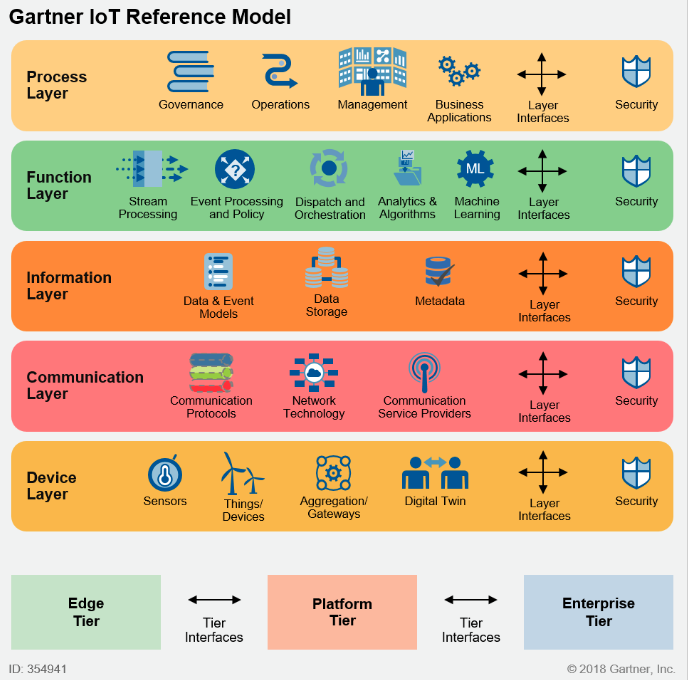
\includegraphics[width=75mm,scale=0.75]{Figures/gartnerIoT}
	\decoRule
	\caption[Gartner]{gartnerIoT1}
	\label{fig:gartnerIoT}
\end{figure}
\section{Prototyping (1-2p)}
//Proof of concept, MvP, Rapid Prototyping
\section{Front-End}
//Should I talk about other options too? (also in the following sections)
Reactjs is an Open-Source Javascript-Libary.
After developing Reactjs in 2011, Facebook soon discovered that it's performance was faster than other implementations of its' kind and made it Open-Source in 2015. 
At present, React is used by major companies for their front-end like Airbnb, Netflix and Reddit \parencite{reactjsUsers}. 
In this years' Stackoverflow-Survey, React came third in "Most Popular Framework, libary or Tool" \parencite{stackOverflowSurvey}. 
This year, over 100,000 developers participated in the survey. 
React is designed for building User-Interfaces. Other libaries % \parencite{reactjsAngularVue} 
use the same concepts but Reactjs is currently the most popular one.
A lot of libaries are available for react. 
It's main concepts are:
\begin{description}
    \item[Components] \hfill \\
    React motivates its' users to write encapsulated components with single responsibilities. Components combine the HTMl-markup and Javscript-functionality of a responsibility. They are supposed to reusability. %erhöhen
    \item[Composition] \hfill \\
    The user can reuse and composite elements as he needs to. The isolated components makes code easier to maintain. 
    \item[Uni-Directional Dataflow] \hfill \\
            Properties should not be changed in other components, but passed down as read-only variables. 
            React doesn't want children to affect their parent components. That makes maintainability easier, as there's a clear downward structure in a well designed React project.
            If a user needs to pass changes to a parent component, it's executed with callbacks, or, for more complicated architecture with a Flux-supporting libary like Redux.
    \item[Virtual Dom]\hfill \\
    A DOM%Reference to Abkürzung 
    is a logical structure of documents in HTML, XHTML, or XML formats. 
    Web browsers are using layout engines to transform or parse the representation HTML-syntax into document object model that we can see in a web browser.
    Usually, when one of these elements changes, the whole structure has to be calculated again. 
    React uses a Virtual DOM as a negiator to enable calculating only the parts that need calculating. That's also possible because of Reacts' isolated component structure.
    \item[JSX]  JSX, short for Javascript XML, is an implementation of Javascript which is usually used to write in ReactJs. 
    It looks a lot like HTML but enables Javascript functionality. Javascript functionalities can be used by putting them in curly brackets ("{}").
\end{description}
\section{Communication}
%Socket.io
Socket.io is a Javascript-Libary designed for realtime communication. 
The server-side is developed for specifically for Node.js wheras for the client different implementations (e.g. .Net, Swift, C++)\parencite{socketioClients} are available.
It enables a bi-directional communication channel between a client and a server and offers a fallback mechanism to long polling when WebSockets are not available.
Once a connections is established it's maintained and uses a diminishing small amount resources to communicate. 
It uses an event-based system where one participant listens and another emits an event. 
Both Client and Server can emit and listen for events.
\section{Middleware}
%Talk about Node.js
Node.js is an open-source, cross-plattform, javascript-runtime-enviroment. 
With 49.6\% it is this years "Most Popular Framework, Libary or Tool" on this years Stackoverflow-survey \parencite{stackOverflowSurvey}.
According to Google Trends, interest is rising since 2012\parencite{gogleTrendNode}.
One explanation for that might be that it's written in Javascript. 
The transation for front-end Javascript developers to developing back-end is eased, which saves companies learning costs.
Node.js is estimated to have a high learning curve \parencite{nodeLearningcurve}.
It uses an event-driven architecture which operates on a single threaded event loop using non-blocking I/O calls.
Commands use callbacks to signal they are completed or failed. 
A downside is, that it doesn't allow vertical scaling by increasing the number of CPU cores of the machine it is running on. 
On CPU-intensive applications, that might become a problem - but modules like IPC or pm2 can add that functionality.
Node.Js commands are non-blocking and execute concurrently or in parallel. 
It's build on the Google V8 JavaScript engine which compiles Javascript to machine code instead of interpreting it in real time. 
That makes it faster than (some) other engines.
There are thousands of open-source libaries and web frameworks available for Node.js. 
\section{Device}
%Talk about Arduino implementation
Arduino is a microcontroller-company from italy which was founded in 2005. 
It is is completely open source and provides it's own Integrated Development Enviroment(IDE) \parencite{arduinoIDEDownload}.
The IDE works with nearly all microprocessors on the market. 
The IDE recommends a structure for all Arduino programs:
\begin{description}
    \item [Initialization]
    Prior to any function, libaries and necessary variables are declared within an Arduino program.
    \item [setup()]
    The setup-function is the first function called in any Arduino-program.
    \item [loop()]
\end{description}
The Arduino (and comperable microprocessors) are programmed in C.
\section{Back-End}
%Talk about postgres
Postgres is a light-weight open-source object-relational database system. 
Companies like Netflix, Spotify or Instagram \parencite{postgresUsers} rely on the flexible database system which allows SQl and noSQL design.
It's easy to set-up and maintain. 


%Even though, only 26\% of IoT-Projects in companies are judged to be a complete success 
%\parencite{ciscoresearch}. The reasons are as numerous as they are diverse. 
%Lack of knowledge, lack of planning, inconsistent standards and legacy architectures within the project are only some mentioned by the Cisco survey.
%A McKinsey report \parencite{mcKinsey} in 2015 stated that most IoT adopters fail to use their data or derive just a small part of its value.

% Chapter Template

\chapter{Related Work} % Main chapter title

\label{Chapter2} % Change X to a consecutive number; for referencing this chapter elsewhere, use \ref{ChapterX}

%General explanation: We have an escape room that is currently a WSN with only little data processing, we watn to extend the middleware
% to achieve a broader spectrum of integration possibilities.
As explained in Chapter \ref{Chapter1}, the goal of this project was to extend the existing project.
Therefore, possible architectures and practices to integrate to the project were investigated.
In the following, research concerning the development of our project is listed and explained.

\section{Design Thinking}
Design thinking is one strategy to plan an innovation process. 
It seemed to fit the working process and was a guide concerning the production phase, further explained in Chapter\ref{Chapter4}.
In contrast to mechanical improvements, design thinking tries to emphatize with possible customer needs at all parts of the product.
A few of design thinking's key principles are to 
"engage in early exploration of selected ideas, rapidly modelling potential solutions to encourage learning 
while doing, and allow for gaining additional insight into the viability of 
solutions before too much time or money has been spent" and that it 
"Iterates through the various stages, revisiting empathetic frames of mind and then redefining the challenge as new knowledge and insight is gained along the way." 
\parencite{designThinking}
The Stanford Design School, now known as the Hasso Plattner Institute of Design began teaching a design thinking process 
with the three steps of understanding, improving and applying a product. 

Since then, their approach to design thinking moved on to a widely used, open-sourced 5 stage process \parencite{designThinkingCrashCourse}
consisting of the following items:
\begin{itemize}
    \item [Empathise] \hfill \\
    Emphatising relies on three principles: Observe, engage and immerse with your customers
    \item [Define] \hfill \\
    Stanford recommends to unpack the priorly collected findings "to needs and insights and scope a meaningful challenge \parencite{designThinkingBootleg}
    \item [Ideate] \hfill \\
    Ideation is the stage one should explore ideas in a "wide open" \parencite{designThinkingBootleg}. The goal is to create ideas that some 
    can be picked from to create a prototype.
    \item [Prototype] \hfill \\
    Apart from testing, prototyping for this definition of the design thinking process serves many purposes. 
    According to \parencite{designThinkingBootleg}, one can also profit from prototyping for
    \begin{itemize}
        \item Empathy
        \item Exploration
        \item Inspiration
        \item Testing
    \end{itemize}
    purposes. One can receive a deepend understanding by building a prototype (Empathy), explore multiple concepts faster (Exploration),
    inspire other people for one's ideas (Inspiration) test and refine (Testing). 

    \item [Test] \hfill \\
    The testing is an iterative process where one can refine and gather feedback about the product.
\end{itemize}
Figure \ref{fig:designThinking} illustrates the iterative properties of this model.

\begin{figure*}[h]
	\centering
	\copyrightbox[r]{\includegraphics[width=75mm,scale=0.75]{Figures/designThinking}}{\textcopyright Author/Copyright holder: Teo Yu Siang and Interaction Design Foundation. Copyright terms and licence: CC BY-NC-SA 3.0}
	\caption[designThinking]{}
	\label{fig:designThinking}
  \end{figure*}

The model goes on to describe user analysis methods which are not relevant in the context of this project, 
since the project prioritized the development of a working prototype over extensive user studies. 

\section{Prototyping (1-2p)}
A prototype is "An initial model of an object built to test a design." \parencite{prototypeDef}
A favored approach to prototyping within the IoT-scape is "Rapid Prototyping" 
which favors fast production cycles over extensive feature development. 
As S. Hodges states, "By prototyping and deploying live systems early on in the concept development cycle it is possible to understand the strengths and weaknesses of a particular application, design or specific implementation sooner 
and feed this information back into an iterative development process." \parencite{rapidProto3}
The same paper introduces .NET Gadgeteer, which was a rapid prototyping platform developed by Microsoft but is no longer maintained since 2016.
The idea of Gadgeteer was to introduce a plug-and-play mechanism to IoT-development, where the developer had to connect the devices on a visual interface and code would be generated automatically.
Due to it's high initial cost (250\$ for a starter kit), 
and it's incompatibility with other shields it was not competitive against the Netduino or the Arduino platform explained in the "Device"-section below.
Two generally important concepts in a product lifecycle surrounding a development process 
are the "Proof of Concept" and the "Minimal Viable Product".

\subsection{Proof of Concept}
The business dictionary defines a proof of concept as "Evidence which establishes that an idea, invention, process, or business model is feasible."
\parencite{PoC}
A proof of concept can take many forms depending on the product and the industry it develops in. 
In a technological environment, proof of concept often take the form of prototypes defined by a set of goals.

\subsection{Minimal Viable Product}
A minimival viable product (MVP) is a product with "sufficient features to satisfy early adopters" \parencite{mvp}. 
Only after considering feedback by customers is the product developed further. 
MVPs allow companies to publish a product as early as possible which leads to early monitary profit and fast feedback. 
On this basis, user
The concept has been popularized by Eric Ries, a consultant of start-ups.

\section{Architecture (2-3p)}

As there is, at this point in time, no consensus reached for a layer model defined for IoT-architectures \parencite{noModel}
different approaches can be used to analyze and structure an IoT-system. 
The following describes three proposed layer-models.

\subsection{Gartner IoT architecture}

This project adapted Gartner's take on IoT architecture as it offers a powerful and complex overview about different 
possibilities of IoT integration. 
It offers an architecture as well as a taylored layer model.

\begin{figure}[th]
	\centering
	\includegraphics[width=100mm,scale=1]{Figures/gartnerIoT2}
	\decoRule
	\caption[Gartner]{Tiers of the Gartner IoT architecture}
	\label{fig:gartnerIoT2}
\end{figure}

\begin{description}
    \item[Edge Tier]\hfill \\ 
    The left part of Figure \ref{fig:gartnerIoT2} depicts the edge tier of an IoT-architecture.
    The "Edge Tier" is where sensors and actuators lie.
    Wheras a sensor \textit{detects} interaction or changes in a physical environment, an actuator is
    "a device that is used to \textit{effect} a change in the environment" such as the temperature 
    controller of an air conditioner \parencite{archsurv4}. 
    Sensors and actutators typically complement each other.
    The figure describes 3 general forms the edge can take. 
    It is always a combination of sensors/actuators with either:
    \begin{enumerate}
        \item A "smart" IoT device which pre-processes data before it sends data to the device gateway service
        \item An IoT device with an edge gateway physically connected which transmits the devices data to the device gateway service
        \item A simple IoT device which connects to the device gateway service directly without pre-processing the data from the sensors/actuators
    \end{enumerate}
    
    \item [Platform Tier] \hfill \\
    The middle part of Figure \ref{fig:gartnerIoT2} shows the platform tier of an IoT-architecture.
    According to Gartner, the pre-processed or raw data from the edge is processed here. %%verarbeitet
    Stream processing, event handling and database implementation take place.
    Additionaly, edge devices can be overseen with monitoring tools integrated. 
    If needed, further requirements for enterprise authentification and handling are also implemented at that layer.
    Summing up, this layer is responisble for all data-managment tasks that might arise in an IoT-system.


    \item [Enterprise Tier] \hfill \\
    The "Enterprise Tier", depicted on the right, is the customer part in an enterprise solution for IoT-architectures.
    It provides the customer with necessary data in a pleasant and clear way.
    While the customer has access to the platform layer through the application layer, he doesn't get in touch with the platform layer directly.  %übersichtlich 
\end{description}

\begin{description}
    \item[Device Layer] \hfill \\
    The Device Layer is the phyiscal layer in this model. 
    It owns the Edge Tier properties, sensors, actuators and respectively one of the three extending devices. 
    According to Gartner, this is the recommended layer to start when planning an IoT-architecture, as it defines the bandwidth of devices that need 
    to communicate with a gateway and therefore the communication protocols that work with it in the long run.
    If an edge gateway is present, it's also part of the Device Layer.
    \item[Communication Layer] \hfill \\
    This layer defines how the communication is taking place within an IoT-system.
    Depending on the Devices within the system, different communication protocols and data models should be implemented.
    Examples of IoT-protocols are MQTT, Wi-Fi, WPanO6, Zigbee, 
    wheras data models include Apples HomeKit Database, the open-source OpenHab Things model or the SmartThings Capabilities model by Samsung. 
    Different models work with different protocols, 
    so possible future device implementations must be considered.
    \item[Information Layer]  \hfill \\ 
    The Information layer defines how the data is \textit{formatted so it can be interpreted}.
    Depending on the protocols and data models chosen in the Communication Layer, 
    different strategies to format messages by devices can be applied.
    Endpoint and edge identification is important to access different features provided by a Device.
    The messages need to be interpretable possibly by various Devices.
    \item[Function Layer] \hfill \\ 
    The Function Layer is the core of any IoT-application.
    It handles event processing, stream processing, analytics and possibly machine learning.
    Any middleware and back-end tasks are handled here.
    \item[Process Layer]   \hfill \\
    The Process Layer is the front-end in this Layer Model. Proccessed data can be displayed and managed by a user. 
    Depending on the use case, several process layers can belong to one IoT-system (e.g. one for a device manager, and one for displaying data).
\end{description}

\begin{figure}[th]
	\centering
	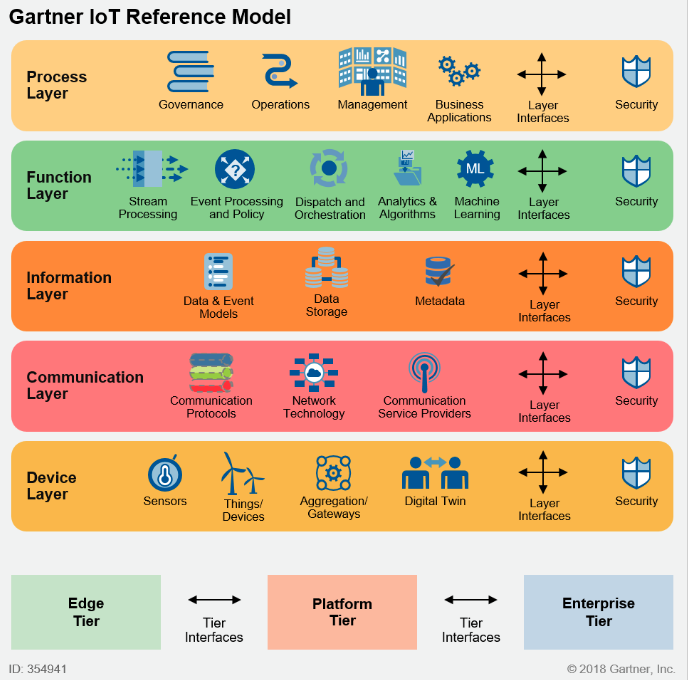
\includegraphics[width=100mm,scale=1]{Figures/gartnerIoT}
	\decoRule
	\caption[Gartner]{Gartner Layer Model}
	\label{fig:gartnerIoT}
\end{figure}



\subsection{Five-Layer architecture}
One by \parencite{fiveLayer1,fiveLayer} proposed model is a five-layer-model consisting of the following layers.
\begin{description}
    \item [Perception layer] \hfill \\
    The perception layer is the physical layer of the architecture. Sensors and actuators exist in this layer.
    \item [Transport layer] \hfill \\
     The transport layer transports data from the perception layer to the processing layer. Different network protocols can be used
   \item [Processing layer] \hfill \\
   The processing layer stores, analyzes and channels incoming data. It is also known as the middleware layer.
   \item [Application layer] \hfill \\
   The application layer is responsible for delivering user-relevant data to a user.
   \item [Business layer] \hfill \\
   The business layer manages the whole system, e.g. applications, business and profit models.
\end{description}


When talking about IoT-architectures, one should mention the difference between cloud and fog/edge based architectures. 

Cloud based architectures assume that processing and analyzing of data should happen in an enviroment remote from the devices' location.
The network below sends data to the cloud, and above the cloud lie applications working with the processed data with the cloud in the center of this architecture.
In the last years, cloud computing has gained popularity, also in the context of IoT architectures \parencite{CloudComputing} because it provides great exibility and scalability.

A newer trend instead are fog or edge based architectures, where the sensors and gateways do parts of the data processing and analytics.
A fog architecture \parencite{FogComputing1, FogComp} presents a layered approach, inserting various layers between the physical (perception) and transport layers 
(monitoring, pre-processing, storage, security). 
Wheras fog computing refers to smart sensors and gateways, edge computing refers to not-smart objects like motors, pumps with 
smart data preprocessing capabilities \parencite{edgeFog}.


\section{Front-End}
As \parencite{frontendDef} states:
"A front-end system is part of an information system that is directly accessed and interacted with by the user to receive or 
utilize back-end capabilities of the host system. 
It enables users to access and request the features and services of the underlying information system."  

The front-end is the visual component of any application. 

Disciplines like UX (User Experience), UI(User Interface) and  IxD (Interaction design) have been working on creating 
a "better" front-end-experience for many years. 

Usually, a mixture of HTML, CSS and Javascript is used for front-end development. 
In recent years, libaries that combine HTML and Javascript capabilities like React.js, Angular or Vue %\parencite{reactjsAngularVue} 
have been designed to support a component based architecture. 

For this project, React.js was used. React.js will further be called by it's commonly referred name "React".
React is an Open-Source Javascript-Libary.
After developing React in 2011, Facebook soon discovered that it's performance was faster than other implementations of its' kind \parencite{benchmarkReact}and made it Open-Source in 2015. 
At present, React is used by major companies for their front-end like Airbnb, Netflix and Reddit \parencite{reactjsUsers}. 
In this years' Stackoverflow-Survey, React came third in "Most Popular Framework, Libary or Tool" \parencite{stackOverflowSurvey}. 
This year, over 100,000 developers participated in the survey. 
A lot of libaries are available for React. 
Its main concepts are:


\begin{description}
    \item[Components] \hfill \\
    React motivates its users to write encapsulated components with single responsibilities. Components combine the HTML-markup and Javscript-functionality of a responsibility. 
    They are supposed to increase reusability. %erhöhen
    \item[Composition] \hfill \\
    The user can reuse and composite elements as he needs to. 
    The isolated components make code easier to maintain. 
    \item[Uni-Directional Dataflow] \hfill \\
            Properties should not be changed in other components, but passed down as read-only variables. 
            React doesn't want children to affect their parent components. That makes maintainability easier, as there's a clear downward structure in a well designed React project.
            If a user needs to pass changes to a parent component, it's executed with callbacks.
    \item[Virtual Dom]\hfill \\
    A Document Object Model (DOM) is a logical structure of documents in HTML, XHTML, or XML formats. 
    Web browsers are using layout engines to transform or parse the representation HTML-syntax into document object model that we can see in a web browser.
    Usually, when one of these elements changes, the whole structure has to be calculated again. 
    React uses a Virtual DOM as a negiator to enable calculating only the parts that need calculating. That's also possible because of Reacts' isolated component structure.
    \item[JSX] \hfill \\
    %ÜBERARBEITEN
    //ÜBERARBEITEN 

    Javascript XML (JSX), is a Javascript extension of Javascript which is usually used to write in ReactJs. 
    It looks a lot like HTML but enables Javascript functionality. 
    Javascript functionalities can be used by putting them in curly brackets ("{}").
\end{description}
\begin{figure}[b]
	\centering
    \includegraphics[width=125mm, scale=1.25]{Figures/ReactExampleFullsize}
	\decoRule
	\caption[React1]{React example code}
	\label{fig:reactEx}
\end{figure}

\begin{figure}[t]
    \centering
	\includegraphics[width=75mm,scale=0.75]{Figures/EditExample1}
	\decoRule
	\caption[ReactEx]{Resulting Output of example code}
	\label{fig:resultReact}
\end{figure}


\section{Communication}
%Socket.io
There are different ways to communicate between clients and middleware. 
Communication on the web is usually unsynchronized. 
That means that the client requests something and the server responds. 
Problems arise if real-time communication is required. 
Chat-applications e.g. shouldn't require the user to reload a page anytime he wants to see a new message.
Those services demand a more reactive and immediate communication.

For this, web development techniques like AJAX \parencite{ajax} were invented. 
Here, the client requests data automatically, establishing a new connection to the server.

This technique needs a client to request new content instead of listening 
for new information which creates unnessecary overhead and a higher latency than other communication enviroments like websockets.  
 
Websockets pursue this task by creating a bilateral environment for clint-server-exchange. 
This way, the client doesn't need to connect again and again, but listens for events. 
Now-a-days, most browsers are websocket compatible.

For this project, Socket.io was used for client-middleware-communication.

Socket.io is a Javascript-Libary designed for realtime communication build on top of a websocket-protocol.
It enables a bi-directional communication channel between client and server and offers a fallback mechanism to long polling when websockets are not available.
There are several fallback mechanisms available that are determined dynamically by Socket.io:
\begin{itemize}
    \item Websocket
    \item Adobe Flash Socket
    \item AJAX long polling
    \item AJAX multipart streaming
    \item Forever Iframe
    \item JSONP Polling
\end{itemize}

The server-side of Socket.io is developed  specifically for Node.js wheras for the client different implementations (e.g. .Net, Swift, C++)\parencite{socketioClients} are available.
Once a connections is established it's maintained and uses a diminishing small amount resources to communicate. 
It uses an event-based system where one participant listens and another emits an event. 
Both Client and Server can emit and listen for events.

\section{Middleware}
%Talk about Node.js
Middleware is "software that acts as a bridge between an operating system or database 
and applications, 
especially on a network" \parencite{middlewaredef}. 

As happening in other contexts, 
a Service Orientated Architecture (SOA) approach for middleware 
was proposed in many IoT - architectures from the last few years \parencite{archsurv1}. 
SOA encourages decomposition of a complex system into simpler and isolated components.
Thus, reusability and changeability is increased. 
Especially an IoT-scenario with flexible gateway components and on-going extensions can profit from such 
architecture as changes are demanded frequently.

\parencite{archsurv1}
In this case, Node.js was used as middleware between our client front-end and the database-backend.

Node.js is an open-source, cross-plattform, javascript-runtime-enviroment. 
With 49.6\% it is this years "Most Popular Framework, Libary or Tool" on this years Stackoverflow-survey \parencite{stackOverflowSurvey}.
According to Google Trends, interest is rising since 2012\parencite{gogleTrendNode}.
One explanation for that might be that it's written in Javascript. 
The transition for front-end Javascript developers to developing back-end is eased, which saves companies learning costs \parencite{nodejssavescost}.
It uses an event-driven architecture which operates on a single threaded event loop using non-blocking I/O calls.
Commands use callbacks to signal they are completed or failed. 
A downside is, that it doesn't allow vertical scaling by increasing the number of CPU cores of the machine it is running on. 
On CPU-intensive applications, that might become a problem - but modules like IPC or pm2 can add that functionality.
Node.js commands are non-blocking and execute concurrently or in parallel. 
It's build on the Google V8 JavaScript engine which compiles Javascript to machine code instead of interpreting it in real time. 
%Statistik zu schnelligkeit
There are thousands of open-source libaries and web frameworks available for Node.js. 

\section{Device}
%Talk about Arduino implementation
An IoT-Device can take many forms: 
Sensors and actuators can be used to create nearly any use case, 
from motion detection for light automation, to tracking the productivity of a machine to automated heating depending on room temperature.

\subsection{Arduino}
A popular choice for self-made technology projects is the Arduino microprocessor.

Arduino is a microcontroller-company from italy which was founded in 2005. 
It is completely open source and provides its own Integrated Development Enviroment(IDE) \parencite{arduinoIDEDownload}.
The IDE works with nearly all microprocessors on the market. 
The IDE recommends a structure for all Arduino programs:
\begin{description}
    \item [Initialization]
    Prior to any function, libaries and necessary variables are declared within an Arduino program.
    \item [setup()]
    The setup-function is the first function called in any Arduino-program. 
    This is were variables, supporting hardware or the serialport are initialized and pin modes are set. 
    \item [loop()]
    The loop-function loops consecutively, 
    which enables the program to change and respond on run-time.
    Checking for changes usually happens here, 
    whereas consequences of those changes are implemented outside the loop-function.    
\end{description}
The Arduino (and comperable microprocessors) are programmed in C.

Right now, the Arduino is not the most typical choice for IoT-devices in particular as Arduinos 
with included supporting hardware (e.g. Wi-Fi-modules) released just this year,
however due to it's popularity many libaries and instructions exist to introduce an Arduino to an IoT-scope.
E.g. with additional hardware like a Wi-Fi shield and existing free apps like "Blynk"  \parencite{blynk}, 
an Arduino can be tracked and controlled within 30 minutes of set-up.

\begin{figure*}[h]
	\centering
	\copyrightbox[r]{\includegraphics[width=75mm,scale=0.75]{Figures/adafruitSPI}}{\textcopyright https://learn.sparkfun.com/tutorials/serial-peripheral-interface-spi/all }
	\caption{Visualization of SPI communication}
  \end{figure*}



\section{Back-End}
%Talk about postgres
According to the Oxford Dictionary, a back-end is 
"The part of a computer system, piece of software, etc., where data is stored or processed rather 
than the parts that are seen and directly used by the user" \parencite{backendDef}

If an architecture contains middleware, the back-end is usually responsible for storing and retrieving data for other parts of the system.
Accordingly, a database and a database management system (DBMS) are introduced.
The database stores the data, whereas the DBMS makes the data accessable from elsewhere.
Famous, established examples for DBMS are MySQL and Oracle.
Most DBMS are heavily influenced by the standardised SQL-language which was first introduced in 1970 by Edgar F. Codd in context with the relational model.
An important idea of the relational model is the concept of database normalization, where related records are linked by a key predicate common to all.

For this database, PostgreSQL was used.
PostgreSQL is a light-weight open-source object-relational database system. 
Companies like Netflix, Spotify or Instagram \parencite{postgresUsers} rely on the flexible database system which allows SQl and noSQL design.
It is easy to set-up and maintain. 


%Even though, only 26\% of IoT-Projects in companies are judged to be a complete success 
%\parencite{ciscoresearch}. The reasons are as numerous as they are diverse. 
%Lack of knowledge, lack of planning, inconsistent standards and legacy architectures within the project are only some mentioned by the Cisco survey.
%A McKinsey report \parencite{mcKinsey} in 2015 stated that most IoT adopters fail to use their data or derive just a small part of its value.
 
% Chapter Template
\chapter{Project Overview5-10p} % Main chapter title
%What is the problem and its effects?
\label{Chapter3} % For referencing the chapter elsewhere, use \ref{Chapter1} 
\section{Analysis}

\subsection{Layer Analysis}
%----------------------------------------------------------------------------------------
%	SECTION 1
%----------------------------------------------------------------------------------------
Refering to \ref{fig:gartnerIoT}, we analyzed the existing architecture of the escape room.

\begin{description}
	\item[Device Layer]\hfill \\
	      The Device Layer consisted of multiple Arduinos, and riddle-depending sensors and actuators for each riddle.
	      The gateway device service was an Adafruit Feather 32u4 which is connected via USB to a computer.
	\item[Communication Layer]\hfill \\
	      The communication within the room was set-up with RFM69HCW transceiver modules.\parencite{radiorange}
          The RFM69HCW is very cheap, easy to use and to set-up transceiver. They do packetization, error correction and auto-retransmit which makes them easy to handle.
	      They are designed for point-to-multipoint communication with one transceiver set as a gateway node which sends data to the other transceivers in the room.
	      There are two open-source libaries for the RFM69HCW, the LowPowerlab \parencite{LowPowerLab} and Radiohead \parencite{radiohead} libary.
	      The escape room used the LowPowerlab libary since the architect who designed the room prior to our adjustments was familiar with the libary.
          Now-a-days the Radiohead libary is the recommended libary \parencite{adafruitRecommends} since it's documented more thorough by an active community, kept up-to-date and is cross-platform friendly.
         
          The gateway transceiver was connected via USB to a computer where the data was forwarded via serialport communication (UART).
          In difference to SPI, UART is asynchronous and needs to be made synchronous to be interpreted by an other device. 
          Therefore, a stop- and start-bit is added to any message and transmission speed needs to be set on both sides.
          If the transmission speed differ, the messages can't be interpreted correctly by either side.
            
          Any node (riddle) within the room was recognized by a different nodeID and the gateway detected with a specified "GatewayID". 
        For security-reasons, password-encryption was used between the nodes. 

          The Arduinos within the room connected to the RFM69HCW via Serial Pheriphical Interface (SPI).
          SPI is a serial communication protocol common for micro-processor connection. 
          It uses an extra "Clock" (CLK) line to keep both sides in sync. 
          Only one side generates the clock signal (usually called the "master"). The other side is called the "slave".
          There can be multiple slaves, but only one master.
          The clock is an oscillating signal that tells 
          the receiver when to sample the bits on the data line exactly. 
          Bits are send either on the "high to low" or "low to high" edge of a CLK signal.
          If the master wants to send data to a slave, it's send via a MOSI line, for “Master Out / Slave In”.
          If a slave wants to send data to the master the data will be put on a third line called MISO for "Master In/Slave Out".
          The master will continue to generate a prearranged number of clock cycles, before the message is read by the master.
          As there is a MISO and a MOSI line, full-duplex communication where data is simultaniously send and received is possible with SPI.
          The fourth line needed to enable SPI communication is the "Slave Select"(SS) line which opens the communication channel. 
          If there is only one slave, the "SS" line is kept low (its active state) as long is the device is on. 

          \begin{figure*}[h]
            \centering
            \copyrightbox[r]{\includegraphics[width=75mm,scale=0.75]{Figures/adafruitSPI}}{\textcopyright https://learn.sparkfun.com/tutorials/serial-peripheral-interface-spi/all }
            \caption{Visualization of SPI communication}
          \end{figure*}
          
	\item[Information Layer]\hfill \\
        The Information Layer was build around a simple event model: the transceivers would send codes in a "Number/Number/Number..."-structure. 
        A node could be identified through the string it sent, since the first number would be the node's adressing number. 
        The other numbers would represent the current state of the Arduino with a "Switch-Case" scenario \ref{fig:switchCase}. 
	\item[Function Layer]\hfill \\
        A C++-Server would broadcast all incoming messages to any TCP-Client.    
        The server would forward any messages coming from a TCP-Client back to the serialport just as well.
	\item[Process Layer]\hfill \\
	If the Code matched with the Tcp-Clients list (in our case, in a Unity application), a Video in Unity would be played and Unity would send a "reset" code to the matching riddle. 
    Both lists were defined statically.] 
	Apart form the main functionality, the C++-Server offered a communication window where serialmessages 
    could be seen and sent manually. \ref{fig:c++window}.

\end{description}

    \begin{sidewaysfigure}
        \centering
        \includegraphics[width=200mm,scale=2]{Figures/escapeUmlOld}
        \caption{The old escape room architecture}
        \label{fig:oldEscapeUml}
    \end{sidewaysfigure}

\ref{fig:oldEscapeUml} provides further insight into the architecture

\begin{figure}[th]
    \centering
    \includegraphics[width=75mm,scale=0.75]{Figures/switchCase}
    \decoRule
    \caption[messages]{Example of the messages defined in the Arduino}
    \label{fig:switchCase}
\end{figure}

\begin{figure}[th]
    %\includegraphics[width=75mm,scale=0.75]{Figures/c++window}
    \decoRule
    \caption[messages]{Original Serial Window}
    \label{fig:c++window}
\end{figure}

\subsection{Workload analysis}
%SECTION TWOOO
In 2009, Kim Goodwin stated that 
„Interactive products and services tend to require four different types of work from users: 
cognitive, visual, memory, and physical“ \parencite{designDigitalAge} 
While an IoT-System is not always interactive, the goal of this thesis was very interaction-orientated: 
The goal was to help engineers expand the existing room which would require 
interaction with the Device-Layer (if they wanted to add hardware-functionality) 
and the Process-Layer (if they wanted to add software-functionality).
Therefore it makes sense to analyze this specific project with those aspects in mind. 

It should be mentioned that the room was well designed for the target user, which is an escape room customer, and 
the four areas of cognitive, visual, memory and physical work involved would already be pretty low.
Because this analysis will focus on an engineers point of view, the mentioned user in this case is the engineer who wants to extend or modify the room in some way.

\subsubsection{Cognitive Work}
Engineering products usually demands some kind of cognitive work. Still, there are hurdles that can be avoided,
like finding out wether to click "yes" "no" or "cancel" in a confirmation dialog can be made clearer if the question is phrased easily.
In this case, the cognitive work needed to add a riddle or a functionality was very high:

Device Layer:
\begin{enumerate}
    \item The engineer needs to understand the transport protocol and therefore needs to 
    \begin{enumerate}
        \item Set-Up the RFM69HCW with an Arduino or an Adafruit Feather, which requires drivers and another libary
        \item Understand the communication within the LowPowerlab-libary
        \item Look up the other riddles codes to avoid using a %belegte nodeID
    \end{enumerate}   
    \item Understand Arduino-coding 
    \item Understand working with the "Switch-Case"-scenario used for communication 
\end{enumerate}  

Process Layer:
\begin{enumerate}
    \item Understand C++ to change the Server (f.e. to communicate with an upper-level protocol)
    \item Understand C\# and Low-Level-Socket communication to make changes in Unity 
    and gain an overview about the communication since it's in separate files (one File per Video and one for the Tcp Socket) 
\end{enumerate}  

\subsubsection{Visual Work}
Visual work means how much the user needs to search for features in a product visually.
The visual work within the architecture was low, as the interface to work with was simple.
It didn't offer needed functions for the user, like buttons for often used features(reset, "send feedback"...).

\subsubsection{Memory Work}
Memory work is measured in how much a user has to remember to succeed in a task. 
Typical examples are passwords, command names, and file names.
In its former state, the architecture demanded a high amout of memory work from a developer:
\begin{enumerate}
    \item The developer has to translate "Number/Number/Number..." codes whenever he wants to understand the serialport-messages 
    \item The developer has to remember a different code when he wants to send an order to the device
    \item Anyone who starts the room has to remember to first start the c++ server and afterwards the unity application on the desktop, or connection will fail.
    \item The developer has to enable the "enable feedback" mode for each node manually if he wants to see all messages send
    \item The developer has to enable another mode if he wants to interact with the riddles, and the riddle won't react hardware-wise in that mode.
\end{enumerate} 

\subsubsection{Physical Work}
IoT-Projects always involve some kind of physical work for a developer: the developers need to switch between hardware and software to test the devices for example.
The escape room fits into that scenario but doesn't make testing physically harder than it needs to be in most aspects. 
One aspect that makes changes harder is seemingly unavoidable - most of the hardware is hidden, therefore mostly difficult to access. 
Since an escape room is made for customers who expect the illusion of in this case, a spaceship, 
touch-sensitive hardware would impact that illusion.

% Chapter Template

\chapter{Implementation} % Main chapter title
%Possible solutions (in the context)
\label{Chapter4} % For referencing the chapter elsewhere, use \ref{Chapter1} 

After introducing the project as it existed before this thesis,
this chapter will concern the planning and implementation of the extension that was build.
The implementation used the aforementioned tools as well as some smaller libaries that will be explained in the following section.

\section{Project Design}
The project's design followed a design thinking approach.
The following shows the different steps that were taken that lead to the changes that were planned.

\begin{description}
	\item [Empathise]\hfill \\
	      As a first step, interviews and tests with the existing project were executed.
	      Orignially, the author wanted to build another riddle for the room.
	      It was quickly discovered that constraints would complicate that task.
	      Three people who had worked with the room reported they experienced severe difficulties
	      on trying to change the existing pattern.
	      Frequently mentioned was the overall lack of understanding the room as a whole.
	      Some parts, like the TCP-socket in Unity, were relatively easy to modify, others, like the riddles themselves were disclaimed
	      "not to be touched or they might break".
	      As the room had many visitors (a few a hours a day, 2-4 times a week), changes which would affect the look
	      of the room or make it unstable for a longer period of time were not welcomed.

	      In the time following these interviews,
	      a deeper occupation with the project seemed necessary to develop alternative ideas for this thesis.
	      The author's impression was that the project lacked documentation and explanations on many sides.
	      Understanding the processes and the different parts of communication proved to be difficult,
	      as it didn't seem to follow any standartized structure or protocol.
	      The result of this examination is further explained in Chapter \ref{Chapter3}.

	      On questioning the former architect about his choices,
	      he stated that the project was build under time pressure
	      and everything was therefore implemented best to the architect's knowledge,
	      but without further scientific research or extensive planning.

	\item [Define]\hfill \\
	      The "Empathise" stage lead to the impression that a new riddle
	      would be considered "nice-to-have" whereas
		  extensions to improve the flexibility and comprehensibility of the room would be welcomed.
		  Derived from the workload anyalysis in Chapter \ref{Chapter3},	 
	it was determined that the cognitive and memory work required from a developer were the most critical points
	that one might spend a lot of time on, or might decide not to join the project at all.
	It was defined that:

	To reduce cognitive (C) work, the process of learning and discovering the project must be simplified.

	To reduce the memory (M) work, the amount of commands to remember to control the room must be reduced and the start-up of the room must be simplified.

	\item [Ideate]\hfill \\
	The next step was to devise ideas and to estimate their workload to decide 
	which should be included in the prototype. Since the author had little experience as a software developer,
	complicated coding tasks (judged by the author's supervisor) were cut, 
	like a graph-editor for the front-end.

	After discussing possible approaches, a few specific tasks were set:
	      \begin{enumerate}
		      \item Developing a web interface that would:
		            \begin{itemize}
			            \item Enable more overview and control for the existing riddles (M)
			            \item Ease the testing process for new riddles by displaying them dynamically (C)
			            \item Allow remote access (P) and control (C) within the lokal w-lan enviroment
		            \end{itemize}
		      \item Retrieving information from the room must work automatically, therefore should the "feedback mode" be enabled on start-up (M)
		      \item Providing a thorough documentation for future developers  (C/M)
	      \end{enumerate}

	      The summarized goals for improvement in the different areas can be seen in \ref{fig:workload}.

	      \begin{figure}[th]
		      \centering
		      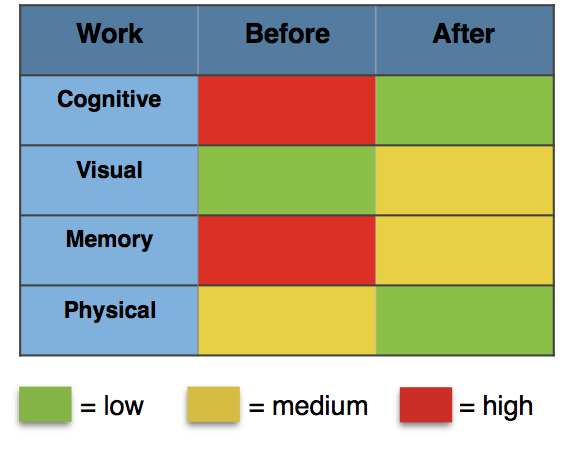
\includegraphics[width=50mm,scale=.5]{Figures/workload}
		      \decoRule
		      \caption[workload]{Workload of the different aspects color-coded}
		      \label{fig:workload}
	      \end{figure}

	\item [Prototype]\hfill \\
		 Afterwards, prototyping began. 
		 The development process of the prototype is explained in the following sections of this chapter.
	    Proof of Concepts were designed for each stage of the implementation (\ref{fig:PoC}).
	\item [Test]\hfill \\
		  Testing happened regulary at least once a month, later every two weeks.
		Extensive testing was difficult to achieve, as the room did not provide 
		   an internet connection needed to install modules (e.g. Node.js) on the PC 
		   and missed basic testing tools like a coding enviroment. 
		   Additionaly, due to the room's physical set-up, testing directly on the PC turned out 
		   to be inconvenient. The PC was hidden behind a wall and difficult to access, 
		   which meant mouse and keyboard could barely reside outside the wall's recess.
		   Consequently, most testing was conducted on two laptops brought by the author: 
		   One Macbook Pro from 2009 with OSX 10.11.6, and a Windows laptop with Windows 10 installed.
		   Throughout testing, new features were designed and iterated.
\end{description}

Our final result is a MVP %Reference abkürzung 
which provides the bare functionalites but lacks in design 
and more extensive features which we will eleborate in the evaluation.

\begin{figure}[th]
	\centering
	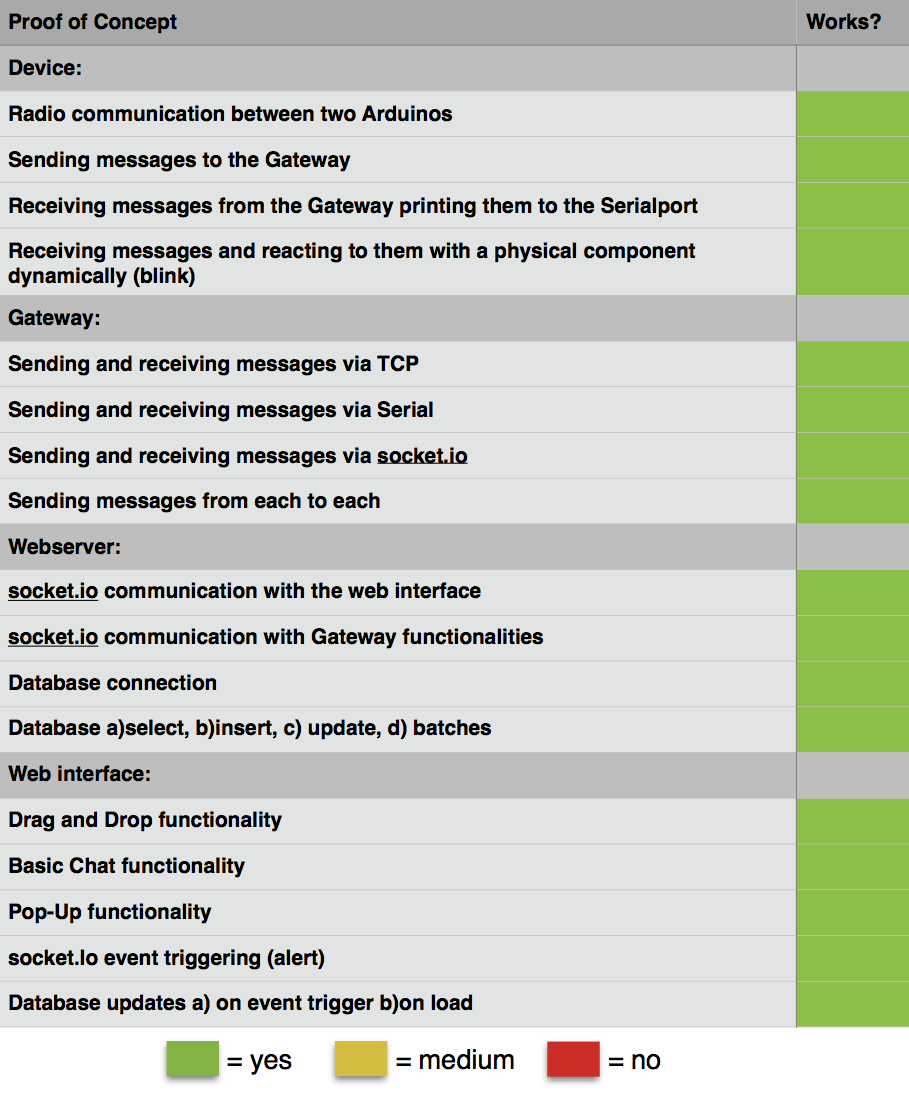
\includegraphics[width=100mm,scale=1]{Figures/PoC}
	\decoRule
	\caption[PoC]{List of our PoC steps}
	\label{fig:PoC}
\end{figure}


\section{Architecture}

As mentioned earlier, IoT-Projects typically follow a SoA %Reference to abkürzung!
to keep the project flexible and expandable.

The goals were set with that architecture in mind and resulting architecture changes
designed to become loosely coupled to encourage improving a specific module of the project.

The changes were meant to reflect concepts of a SoA, creating self-contained,  
reusable and loosely coupled components
to encourage improving a specific module of the project on demand.

For example, the TCP- and serial-connection were set-up in a general way (send/ receive all) 
to separate the data processing from the transport channels. 

Also, communication was designed not interfere with other each other, e.g. 
communication to Unity should still work if a connection to the front-end failed.

For that reason, a backend was implemented which ensured reliable data storage.

In that way, changes reflect the composition of a fog architecture, 
though there is no cloud available or planned which is an important part 
of larger IoT project architecture.

The front-end connection received it's own namespace for Socket.io events so front-end relevant data
would only be proccessed in it's set namespace component.

\begin{sidewaysfigure}
	\centering
	\includegraphics[width=200mm,scale=2]{Figures/escapeUmlNew}
	\caption{The new escape room architecture}
	\label{fig:newEscapeUml}
\end{sidewaysfigure}
%picture of our architecture

\section{Device}
Since the room consisted of microcontroller-driven-riddles only at the time of this thesis, 
we decided to design a prototype and a template for integration of future microcontroller-driven-riddles.
The principle concepts though are appliable to any device.

\subsection{RFM69HCW Wiring}
As most riddles are connected to RFM69HCW modules manually, the first set-up of the prototype 
consisted of an Arduino Uno connected to a RFM69HCW. As one can see in Figure \ref{fig:prototypeV1},
the wiring looks chaotic.



Later, the set-up was replaced with an Adafruit Feather 32u4 which is a microprocessor with an integrated 
RFM69HCW module an therefore reduces the complexity of the wiring needed for the riddle.
This prototype included an external battery as the Feather doesn't support 5V output.
The Adafruit Feather 32u4 needs an external libary to work, the only difference though (apart from the radio set-up)
is the assignment of the SPI lines.

\begin{figure}[H]
	\centering
	\includegraphics[width=75mm,scale=.75]{Figures/prototypeV1}
	\decoRule
	\caption[prototypeV1]{Prototype, Version 1}
	\label{fig:prototypeV1}
\end{figure}


\begin{figure}[H]
	\centering
	\includegraphics[width=50mm,scale=.5]{Figures/prototypeV2}
	\decoRule
	\caption[prototypeV2]{Prototype, Version 2}
	\label{fig:prototypeV2}
\end{figure}

\subsection{Template}

The template was designed to simplify the process of developing a riddle.
The escape room provided in its prior form no support for new riddle-developers.
We decided to modify the existing communication protocol, 
but had to be careful not to impact communication to the existing riddles.

Still, we wanted simplify the communication system for riddle-developers.

The existing communcation protocol followed a "string-to-chararray-send" and "receive -chararray-to-string" structure that we applied to our implementation.
In contrast to the existing puzzles though, we decided to separate the code into several parts, named by the functionality they supplied.

%Chararrays are smaller than strings hence faster for radio-communication.
The template is devided into 3 parts: "Groundwork", "Riddlefunctionality" and "Remote Functionality".

\begin{description}
	\item [Groundwork]\hfill \\
	      Section to be filled with libaries, variables and definitions.
	\item [Riddle Functionality]\hfill \\
	      To contain the riddles functionalities separated from nearly any communication.
	      The only communication that needs to be defined there is when the Microcontroller should send messages and which.
	      That is executed by writing a single line command containing the desired string.
	      If the string's value is defined in the "registerRiddle()" function of the "Remote Functionality" section, it will be translated in the web interface.

	\item [Remote Functionality]\hfill \\
	      To contain any remote commands for interaction with the web interface and the server.
	      The "Remote Functionality" section consists of two functions:
	      \begin{description}
		      \item [registerRiddlle()]\hfill \\
		            Here is where strings to be send once on starting the device are defined.
		            These strings set the configuration of the variables in the web interface.
		            To work, they need to follow a specific structure:
		            \begin{enumerate}
			            \item an Index for the riddlevariable (to order the variables)
			            \item a "readonly" or "write" command (to make it static or dynamic)
			            \item the name of the variable (to translate)
			            \item the value of the variable (needs to be converted into a String)
			            \item an optional button value (if it was present, a button would show)
		            \end{enumerate}
		            That structure is meant to be applieable for any variable.
		      \item[remoteCommand()]\hfill \\
		            Designed to contain processing of incoming messages from the gateway/PC.
		            It's connected to the radio functionality further down in the code, nevertheless allows the user not to care about how the messages are processed.

		            The developer is advised to use a "Switch-Case" structure to define the microcontroller's reactions to radio messages, to keep the processing clean and standartized.
		            For any reaction concerning the defined variables, the case should match the index of the variable in order for the buttons within the web interface to work.

	      \end{description}

\end{description}



\begin{figure}[th]
	\centering
	\includegraphics[width=75mm,scale=0.75]{Figures/registerRiddle}
	\decoRule
	\caption[registerRiddle]{"registerRiddle" definition in the Arduino IDE}
	\label{fig:registerRiddle}
\end{figure}

%fig arduino def

The documentation provided explains the template in further detail.

\subsection{Prototype}

For our prototype, an Arduino Uno with a RFM69HCW module, a keypad, and an I2C-display were used.
All the parts required specific libaries.
%Pictures of syntax and libaries
The riddles challenge would be to guess a code and enter it.
The use case would be that a riddle could to provide different difficulties by adjusting the codes length.
Moreover would the riddle possess static  "won", "lost", and "reset"-values to track and control the riddle's state.
%prototype pic

\section{Back-End}
PostgresSQL was used and the relational model implemented for the back-end.
Two tables were enough to fit our needs.
One table manages the location, name and other general information about the riddle displayed in the main view,
whereas the other one is responsible for saving and editing the information displayed in the pop-up window.
The key predicate was the id of the riddle, which was common to both tables.
This seperation simplifies database changes, clearifying the tasks happening on the Node.js server.
The Node.js server connects the information when sending to the front-end by assigning the details with the riddle's id to the corresponding riddle.

%Database schema einfügen
\section{Middleware}

\subsection{Web Server}
It quickly became apperant that the middleware web server would use Node.js due to the reasons mentioned in \ref{Chapter2}.
The decisive factor for this decision was that it would be easier to develop and understand a web server programmed in the same language as the front-end.

As all the website operations were processed on the client-side, Node.js main operation was the database and handling.
The "pg-promise" libary \parencite{pg-promise} was used for database integration with PostgreSQL.

Depending on the event emitted by the web interface, database-queries to select, update or delete entries could be triggered.

If the gateway emitted a message, a control mechanism would check if the riddle was known and either add a new riddle, update an existing riddle (if new variables where recognized) or translate the incoming data .

With Socket.io, the client would register whether a front-end or another client would register and forward the needed data from the database.
By namespacing (creating different channels for different clients), we tried to avoid dispensable traffic.
The gateway would receive the changeable ("write") values and send them to the connected riddles.
The front-end would receive the sorted database data in a sorted json fit to the front-ends data-handling.

%Architecture We tried to implement our functionalities as loosely as possibilities, so 
\subsection{TCP/Serial/Socket.IO-Client}
This part of the middleware changed several times during our development process.

Since the front-end allowed a reassignement of the messages that would trigger an Unityevent, 
filtering the incoming serial-messages before they were sent to Unity via TCP was required.

Furthermore would they need to be checked for eventual new riddleinformation or messages to be translated or displayed in the front-end.

Consequently, this part of the middleware would filter relevant "Finish"-serialmessages through a PostgreSQL-database, 
and activate a "checkSerialMessage" function which would decide on further processing.

First was tried to use the existing C++-server for the architecture but quickly discovered that understanding and extending the existing code would probably take longer than recreating the features.

Then, because many developers within the faculty were proficient in C\# from Unity development, an implementation the functionalites was tried with a .NET WPF-App.
This proved to be difficult, as it required multi-threading and communication between the threads. 
Both are well documented at the MSDN \parencite{MSDN},
however due to the mass of different techniques it was hard to get an overview.

The resulting code was easier than the C++ code, though not comparable to the readability of the Javascript-code of the Node.js implementation.
It took roughly a week to implement the desired functionalites.

Finally, the  C\# code was revisited and implemented it in Javascript to compare the workload and readability.
The same functionalites took about 10 hours to implement, though the author did by then have little experience in Javascript and started the C\# implementation with Unity-C\#-Knowledge.
The async-capabilities of Node.js revealed a tremendous advantage compared to the threading difficulties experienced with the .NET project in this project.


\begin{figure}[th]
	\centering
	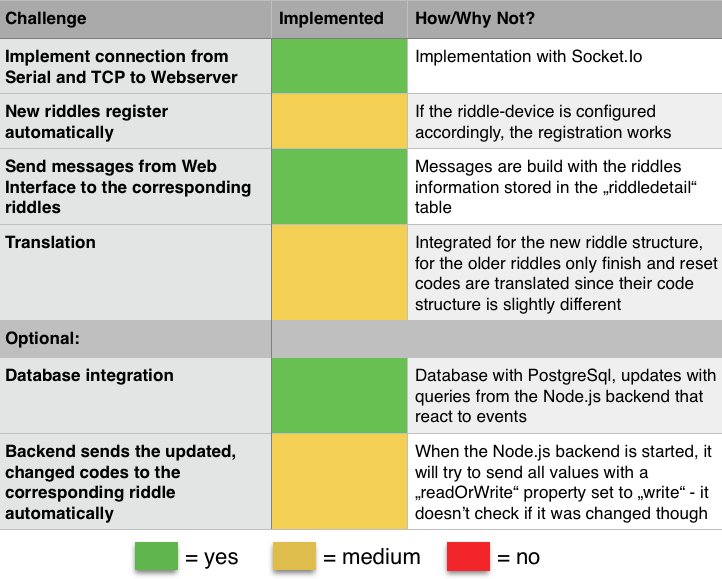
\includegraphics[width=100mm,scale=1]{Figures/backendOverview}
	\decoRule
	\caption[PoC]{Overview of the back-end challenges}
	\label{fig:BackEndTable}
\end{figure}


\section{Front-End}
For setting up our front-end, the Create-React-App was used, which provides a front-end build pipeline with Babel and Webpack.
React recommends to start there for single-page applications \parencite{createReactApp}.

It provides a package.json file in which modules and their versions are defined and set.
This prevents unwanted updates so the existing code won't risk becoming deprecated.

The npm packet manager (which is the standard packet manager for Node.js) automatically generates a package-lock.json file which saves the dependency tree in further detail.

For the file-structure, the recommended approach to group by filetype \parencite{reactStructure} in combination with the Create-React-App-structure was used.
%Fig: Our File structure front end

Starting out, it was planned to implement a node-editor to connect riddles in all thinkable ways.
Wheile listing the wished functionalities (Changeable riddleassignments with "Single", "AND" and "OR" connections to the Unity-Events) it was decided that a drag-and-drop table would supply those functionalites (Changeable assignements, OR connections) without creating a difficult User-Interface.
The React-dnd libary \parencite{reactDND} was used to implement the drag-and-drop functionality in React. 
Currently, it is not mobile-optimized since that was thought to be the less popular use case, but adding a mobile implementation for the module is possible.

When a user dropped a riddle into a "Video" field (and saved), the riddle's "Finish"-command would be reassigned on input to the corresponding Video-Trigger-command.
For example, the "Video1" command was originally triggered by "Riddle1".
If a user wanted to make "Riddle2" trigger "Video1", he needed to replace "Riddle1" in the "Video1"-List with "Riddle2".
Whenever "Riddle2" would now signal it's finished, the "Finish"-code of "Riddle1" would be sent to Unity via TCP.

If a Riddle was newly registered, it would be named "NewRiddle" and appear in the "Unassigned Riddles"-List on the web interface.
We designed an "Edit"-function which enabled changing the name of the riddle and deleting it in case it got corrupted (or deleted in real-life).

Another aspect was the popup-window for the riddles. It was planned to show enough information, yet keep it simple.
Consequently, our layout for the popup-window was designed flexibly to adapt to a desirable output depending on the usecase:

Each variable would be displayed in respect to its in the Arduino defined values.
If a variable was set "readonly", but didn't have a button value defined, the information would be listed plainly.
If a variable was set "write", but didn't have a button value defined, the information would be listed plainly.
Additionaly, an input field would enable changing the defined value and sending it to the Arduino automatically next time the Server would start.

If the microcontroller was programmed to interpret the incoming value, a variable could be changed that way (e.g. a password in a riddle).
If a button component was set in a variable, a button would appear instead of plain information about the variable.
The user would be able to click the button to send the code immediately to the riddle.
This functionality was especially designed with "Finish" and "Start" functionalities in mind, where a supervisor of the escape room might want to trigger these functionalites during a game if customers get stuck.

To increase the general overview for a supervisor, the color of a riddle would change to green once it's "Finish"-code arrived.

\begin{figure}[th]
	\centering
	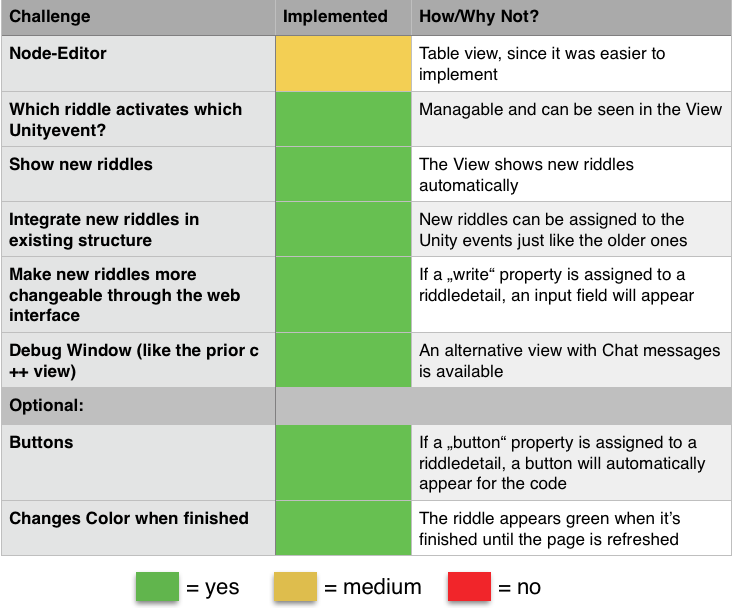
\includegraphics[width=100mm,scale=1]{Figures/frontendOverview}
	\decoRule
	\caption[FrontViewTable]{Overview about our front-view tasks.}
	\label{fig:FrontViewTable}
\end{figure}



 

\chapter{Evaluation and Conclusion} % Main chapter title

\label{Chapter5} % For referencing the chapter elsewhere, use \ref{Chapter1} 

\section{Evaluation}
To evaluate the quality of the changes we made, 
we evaluated the room with the same criterias we picked when judging the room before the changes.

\subsection{Layer Analysis}
Refering to Figure \ref{fig:gartnerIoT} again,the existing architecture of the escape room in respect to the changes we made was analyzed.
\begin{description}
	\item[Device Layer]\hfill \\
	      We didn't make many changes to the Device Layer, as we had instructions not to interfere with the existing structure of the room.
	      Except to adding a prototype implementing the new communication structure, the existing riddles and the gateway Adafruit Feather 32u4 were not manipulated in any way.
	\item[Communication Layer]\hfill \\
	      The Devices do still communicate with RFM69HCW modules and the Low-PowerLab-library via radio communication,
          however, the new webserver functionalities could expand the communication for the software-side of the room. 
          if the server gets a steady network connection.
          An overview from anywhere within the network could be achieved.
	\item[Information Layer]\hfill \\
	      For newer riddles, an advanced communication protocol was developed where a developer of new riddles can use defined strings to trigger events on the device.
	      As the new system should be compatible with the old one, the basis of the communication architecture was not meant to change completely.
	      Instead, the given system of strings separated by a slash ("/") to trigger more actions was expanded.
	\item[Function Layer]\hfill \\
        The Function Layer received the most changes.
        A PostgreSQL database was added to the architecture for filtering and overview purposes.
        A middleware-implementation using the database and Socket.io was established to connect to a front-end using React. 
	      The incoming strings are now translated and send to a web interface.
	      Depending on the string, they trigger a database-query and are interpreted and saved in the database, or update an existing entry.
	      Additionally, the incoming strings are now filtered before they reach the TCP-client(Unity)by the database to ensure proper trigger assignment.
	\item[Process Layer]\hfill \\
          There is now a web interface showing the existing riddles, enabling an immediate interaction with them, 
          and providing a scalable overview about the room.
          Unity triggering is still the main objective of the system.

\end{description}

\subsection{Workload Analysis}
The changed amounts of workload were analyzed again. 
As there wasn't an opportunity to test the findings, the listed views are highly subjective 
and should only be interpeted as the authors impressions, backed by the research mentioned in Chapter \ref{Chapter2}.
\subsubsection{Cognitive Work}
The cognitive work needed to develop parts 
of the software and hardware is expected to be considerably lower with the changes applied.
In the following, prior concerns are compared to our perception now.
\begin{enumerate}
    \item The developer no longer needs to understand the transport protocol in detail
    \begin{enumerate}
        \item 
        He still needs to Set-Up the RFM69HCW with an Arduino or an Adafruit Feather 32u4, 
        which requires drivers and maybe another library, but has thorough instructions through a documentation
        \item doesn't need to understand the communication LowPowerLab library if he uses the designed template
        \item doesn't need to look up the other riddles information as he can look most of it up in the WebInterface
    \end{enumerate}   
    \item Understand Arduino-coding 
    \item Understand working with the "Switch-Case"-communication-protocol used for communication (with instructions)
\end{enumerate}  
Process Layer:
\begin{enumerate}
    \item Understand Javascript to make changes on the server (in a cleaned up, documented and component-based code with improved readability)
    \item Understand Javascript and HTML to make changes to the React-front-end (also component-based) 
    \item     
    There were instructions not to change the Unity application, so the problem of Unity-programming still exists. 
    It would be easier to change though, by replacing the TCP connection with a Socket.io connection. 
    There are multiple client implementations for Unity available \parencite{socketioUnity1, socketioUnity2,socketioUnity3}
    That reportedly work (at least) up to the current version of Unity. 
    Since the Unity version in the escape room won't be upgraded regularily, deprecation issues should not arise.
\end{enumerate}  
\subsubsection{Visual Work}
There was little time to research web-design to an extend where the author could state confidentely that the project's design is especially user-friendly.
Alternatively though, the website offers an improved version of the prior window with an integrated translation of the incoming codes.
Instead of coded strings, the strings are now depicted as readable messages if they are stored in the database.
It also offers a lot more information and possibilites to interact with the enviroment, which reduces the workload in other areas.
\subsubsection{Memory Work}
The memory work is reduced immensely, especially for new riddles. 
The developer has the possibility to save its values as buttons so that he only needs to interact with an abstraction of the machine-code.
\begin{description}
    \item [Buttons] \hfill \\
    By clicking buttons instead of remembering the strings, the developer can take the shortest way to activate a functionality
    \item [Information Display] \hfill \\
    By displaying all riddle information in one place, the developer can gain a better understanding of the riddles functionalities
    \item [Automatisation] \hfill \\
    Tasks like activating the feedback mode of the riddles and sending 
    and starting the applications in the right order were automated.
\end{description}
\subsubsection{Physical Work}
The web server reduced the physical interaction needed to work with the room  silghtly. 
A user can access the room remotely and doesn't need to start the applications manually.

\begin{figure}[th]
	\centering
	\includegraphics[width=100mm,scale=1]{Figures/workTable}
	\decoRule
	\caption[Workload Overview]{Overview about the workload analysis}
	\label{fig:TableWork}
\end{figure}

\subsection{Limitations}
Even though we, to our judgement, achieved our set goals, 
we should mentions the limitations our project might have suffered from.

We were working with an already existing project which we were instructed not to change from its core. 
Instead of designing a new architecture by scratch, we acted therefore within the given frame. 
An architecture from scratch would e.g. have used a simpler communication system for the Arduinos and would have changed 
the Unity communication to an event-based, more dynamic protocol.  

Due to the current Unity communication, resetting the riddles depending on their assignement
is currently not possible, and riddles might be involuntary resetted on activating a trigger in Unity.

The code of the project was build within a 3-month period by the single, unexperienced author.
The most thorough research can not replace hands-on experience, 
just like the most motivated person can usually not substitute the intertwined ideas a team can develop over a course of time.

Because of the tight schedule, there wasn't time to evaluate the user-experience with the new system so the value the framework produces can only be estimated.
Also, lots of features are still missing, listed in the "Future Work"-section below.
A more finished product would have been desirable.


\subsection{Future Work}
This section is meant to list possible ways to expand the built framework.
\begin{description}
    \item [Fully Event-Based-Processing]\hfill \\ 
    By replacing the TCP-Connection to Unity with a Socket.io client, 
    one could take the entire processing to the Node.js server. 
    Since the Node.js server handles the database-queries,
    the events would scale dynamically. 
    Developers wouldn't need to change the Unity code manually everytime a riddle is added. 
    Possible use cases are:
    \begin{enumerate}
        \item Resetting the room could be implemented by selecting all riddle details with "Finish" as an infovalue when Unity sends a "resetRiddles" event.
        \item 
        Resetting the riddle that activated an event in Unity could be implemented by storing the incoming "Finish" 
        value and retrieving its fitting "Reset" value with the ID of the string.
    \end{enumerate}
    \item [Node Editor]\hfill \\
    Developing the front-end further, one could implement a node-editor to create reaction-chains. 
    Such a reaction chain could be that a riddle changes the color of the floor when it's finished by combining two buttons. 
    The data already exists as JSON in the front-end, but creating a flexible drag-and-drop interface with the internal processing 
    went beyond the scope of the project. 
    \item [Security] \hfill \\
    Within the scope of this project, security protection like password authentication and encryption was not included.
    Since the web server is hosted in a local network in a password protected enviroment we didn't prioritize an authentication system.
    Another aspect was that an escape room doesn't contain privacy sensitive data in our point of view.
    \item [Component Isolation]\hfill \\
    Though it was tried to keep the components separated, there is always room for improvement. 
    Especially the Node.js middleware shows room for further splitting and transparency.
    \item[Gateway Configuration]\hfill \\
    As changes didn't affect the communication protocol, scalability issues might arise depending on the number of incoming messages at the gateway component, 
    especially in combination with the current serialport communication. 
    The serial port's UART is running with 9600 baud (which represent the bits per second communicated), 
    960 byte/s, whereas the RFM69HCW is able to send 300kb/s. 
    That's an avoidable bottleneck, if UART were replaced with SPI.
    Alternatively, the baud rate could be increased.
    A Raspberry Pi could be set up as a server with a Wi-Fi module. 
    There is an regulary updatet (last update is 6 months old in a branch) python wrapper \parencite{raspberrypiLibRFM} with thorough documentation \parencite{raspberrypiDoc} available for connecting 
    a Raspberry Pi to a RFM69 module running with the LowPowerLab library. 
    The Raspberry could host the websever in a local, protected Wi-Fi environment and 
    supply the server hosting Unity with the needed events within the closed network. 
    Ideally, Unity would have an implemented Socket.Io connection by then.
    This way, only authenticated users would have access to the escape rooms properties, 
    the architecture would be separated and therefore clearer for developers, and easier to change.
     \parencite{raspberrypiDoc}
     \item[Mobile integration]\hfill \\
     With the webserver running, mobile devices like cellphones or tablets could communicate with the server via Socket.io. 
     This introduces a whole new world riddles that could interact with the cellphone. 
     One could build an alternative front-end for customers, and e.g.
     let them scan something with their camera trough the webpage they access.
     The database could provide further information to a riddle, if e.g. a code should be adressed.
     \item[Smart Capabilities]\hfill \\
     A smart room with more riddles and tracking functionalities would be gratifying.
     Immersion in an escape room can be increased by tracking body functions,
     One could track body functions like heartbeat when controlling 
     the spaceship to start individual audio messages (approval, motivation, disapproval)
     enviromental factors like the temperatue of the room could impact the story telling ("Brrr It's cold in here"/"It's getting hot in here" - audiomessages)


\end{description}
//Picture of Planned architecture (Raspberry, webserver to unity bla)

\subsection{Big Picture}

In the context of other IoT implementations, a rather unusual approach was taken, reasoned with the initial set-up of the room.
Researching, little IoT-implementations apart from the LowPowerLab framework were found with the RFM69HCW module. 
Though it serves it's purpose well, beeing cost-effective, consuming very little power and beeing fairly reliable,
other communication protocols would have been easier to implement and are more flexible in the long-run.
For example a related module which costs 5 euros more, the RFM9X, is becoming popular with the rise of LoRa-WAN in IoT technology. 
LoRa-WAN enables easy access to a Web-Interface with The Things Network (TTN) \parencite{TTN}.
It would also simplify testing, as any "Thing" integrated in TTN can access the gateway within a 2-5 mile range within a city. 
Protocols like Zigbee and LowPower-Bluetooth are an alternative for short-range communication and offer other 
advantages like ZigBees mesh-communication or BLE's easy cellphone communication.
More popular protocols offer more support by a community and are therefore easier to access and update.
That might be on the one hand due to the 
we supplied little hardware extensions.


\section{Conclusion}
%Summarize all main points and insights/discoveries
This project extended the functionalities of an existing escape room.
A framework which might help future developers in integrating new riddles was developed.
We hoped to set a basis for a smart escape room with the new features.


Struktur:
"Why should anybody care"


mobile integration would be possible by accessing the node.js server via socket.io
Erster schritt richtung smart escape room

Narration gets more immersive if a room can react to enviromental factors with sensors. 
Body functions could be tracked for specific tasks, while the room could react to the general status of the room. 
If the room "knows" how many riddles were done, the temperature of the room, 
the number of people within the room, where everybody is with motion or touch detection, it can react appropriately.
Currently, escape rooms need a supervisor to send hints to people within the room. 
A fully developed smart escape room.

%Since the layers of an IoT system are neither standartized nor clear depending on the things included in the network system,
%a layered approach can only be striven for in the execution of a PoC. 


%----------------------------------------------------------------------------------------
%	THESIS CONTENT - APPENDICES
%----------------------------------------------------------------------------------------

\appendix % Cue to tell LaTeX that the following "chapters" are Appendices

% Include the appendices of the thesis as separate files from the Appendices folder
% Uncomment the lines as you write the Appendices

%% Appendix A

\chapter{Frequently Asked Questions} % Main appendix title

\label{AppendixA} % For referencing this appendix elsewhere, use \ref{AppendixA}

\section{How do I change the colors of links?}

The color of links can be changed to your liking using:

{\small\verb!\hypersetup{urlcolor=red}!}, or

{\small\verb!\hypersetup{citecolor=green}!}, or

{\small\verb!\hypersetup{allcolor=blue}!}.

\noindent If you want to completely hide the links, you can use:

{\small\verb!\hypersetup{allcolors=.}!}, or even better: 

{\small\verb!\hypersetup{hidelinks}!}.

\noindent If you want to have obvious links in the PDF but not the printed text, use:

{\small\verb!\hypersetup{colorlinks=false}!}.

%\include{Appendices/AppendixB}
%\include{Appendices/AppendixC}

%----------------------------------------------------------------------------------------
%	BIBLIOGRAPHY
%----------------------------------------------------------------------------------------
\listoffigures % Prints the list of figures


\printbibliography[heading=bibintoc]

%----------------------------------------------------------------------------------------

\end{document}  
